% \subsection{Balanced Neighborhoods}

% \noindent Bias and fairness in machine learning are topics of considerable recent research interest~\cite{pedreshi2008discrimination,fairness,bozdag_bias_2013}. A standard approach in this area is to identify a variable or variables representing membership in a protected class, for example, race in an employment context, and to develop algorithms that remove bias relative to this variable. See, for example, ~\cite{zemel2013learning,kamishima2012fairness,kamiran2010discrimination,zhang2017anti}.

% To extend this concept to recommender systems, we must recognize the key role of personalization. Inherent in the idea of recommendation is that the best items for one user may be different than those for another. It is also important to note that recommender systems exist to facilitate transactions. Thus, many recommendation applications involve multiple stakeholders and therefore may give rise to fairness issues for more than one group of participants~\cite{abdollahpouri_recommender_2017}.

% \subsubsection{Personalization}

% The dominant recommendation paradigm, collaborative filtering, uses user behavior as its input, ignoring user demographics and item attributes~\cite{koren2015advances}. However, this does not mean that fairness with respect to such attributes is irrelevant. Consider a recommender system suggesting job opportunities to job seekers. The operator of such a system might wish, for example, to ensure that male and female users with similar qualifications get recommendations of jobs with similar rank and salary. The system would therefore need to defend against biases in recommendation output, even biases that arise due to behavioral differences: for example, male users might be more likely to click optimistically on high-paying jobs.

% Defeating such biases is difficult if we cannot assert a shared global preference ranking over items. Personal preference is the essence of recommendation especially in areas like music, books, and movies where individual taste is paramount. Even in the employment domain, some users might prefer a somewhat lower-paying job if it had other advantages: such as a shorter commute time, or better benefits. Thus, to achieve the policy goal of fair recommendation of jobs by salary, a site operator will have to go beyond a personalization-oriented approach, identify key outcome variables such as salary, and control the recommendation algorithm to make it sensitive to these outcomes for protected groups.

% \subsubsection{Multiple stakeholders}

% As the example of job recommendation makes clear, a recommender system is often in the position of facilitating a transaction between parties, such as job seeker and prospective employer. Fairness towards both parties may be important. For example, at the same time that a job recommender system is ensuring that male and female users to get recommendations with similar salary distributions, it might also need to ensure that jobs at minority-owned businesses are being recommended to the most desirable job candidates at the same rate as jobs at white-owned businesses.

% A \textit{multistakeholder recommender system} is one in which the end user is not the only party whose interests are considered in generating recommendations~\cite{soappaper,abdollahpouri_recommender_2017}. This term acknowledges that recommender systems often serve multiple goals and therefore a purely user-centered approach is insufficient. Bilateral considerations, such as those in employment recommendation, were first studied in the category of \textit{reciprocal recommendation} where a recommendation must be acceptable to both parties in a transaction~\cite{akoglu_valuepick:_2010}. Other reciprocal recommendation domains include on-line dating~\cite{reciprocal}, peer-to-peer ``sharing economy'' recommendation (such as AirBnB, Uber and others), on-line advertising \cite{targetadvertisingbiding}, and scientific collaboration~\cite{lopes2010collaboration,tang2012cross}.

% When recommendations must account for the needs of more than just the two transacting parties, we move beyond reciprocal recommendation to multistakeholder recommendation. Today's web economy hosts a profusion of multisided platforms, systems of commerce and exchange that bring together multiple parties in a marketplace, where the transacting individuals and the market itself all share in the transaction~\cite{evans_matchmakers:_2016}. These platforms must by design try to satisfy multiple stakeholders. Examples include LinkedIn, which brings together professionals, employers and recruiters; Etsy, which brings together shoppers and small-scale artisans; and Kiva.org, which brings together charitably-minded individuals with third-world entrepreneurs in need of capital.

% \subsubsection{Stakeholder utility}

% Different recommendation scenarios can be distinguished by differing configurations of interests among the stakeholders. We divide the stakeholders of a given recommender system into three categories: consumers $C$, providers $P$, and platform or system $S$. The consumers are those who receive the recommendations. They are the individuals whose choice or search problems bring them to the platform, and who expect recommendations to satisfy those needs. The providers are those entities that supply or otherwise stand behind the recommended objects, and gain from the consumer's choice.\footnote{In some recommendation scenarios, like on-line dating, the consumers and providers are same individuals.} The final category is the platform itself, which has created the recommender system in order to match consumers with providers and has some means of gaining benefit from successfully doing so. 

% Recommendation in multistakeholder settings needs to be approached differently from user-focused environments. In particular, we have found that formalizing and computing stakeholder utilities is a productive way to design and evaluate recommendation algorithms. Ultimately, the system owner is the one whose utility should be maximized: if there is some outcome valued by the recommender system operator, it should be included in the calculation of system utility. 

% The system inevitably has objectives that are a function of the utilities of the other stakeholders. Multisided platforms thrive when they can attract and retain critical masses of participants on all sides of the market. In our employment example, if a job seeker does not find the system's recommendations valuable, he or she may ignore this aspect of the system or may migrate to a competing platform. The same is true of providers; a company may choose other platforms on which to promote its job openings if a given site does not present its ads as recommendations or does not deliver acceptable candidates.

% System utilities are highly domain-specific: tied to particular business models and types of transactions that they facilitate. If there is some monetary transaction facilitated by the platform, the system will usually get a share. The system will also have some utility associated with customer satisfaction, and some portion of that can be attributed to providing good recommendations. In domains subject to legal regulation, such as employment and housing, there will be value associated with compliance with anti-discrimination statutes. There may also be a (difficult to quantify) utility associated with an organization's social mission that may also value fair outcomes. All of these factors will govern how the platform values the different trade-offs associated with making recommendations.

% \subsection{Multisided fairness}

% Recommendation processes within multisided platforms can give rise to questions of multisided fairness. Namely, there may be fairness-related criteria at play on more than one side of a transaction, and therefore the transaction cannot be evaluated simply on the basis of the results that accrue to one side. There are three classes of systems, distinguished by the fairness issues that arise relative to these groups: consumers (C-fairness), providers (P-fairness), and both (CP-fairness).

% \subsubsection{C-fairness}

% A recommender system distinguished by C-fairness is one that must take into account the disparate impact of recommendation on protected classes of recommendation consumers. In the motivating example from~\cite{fairness}, a credit card company is recommending consumer credit offers. There are no producer-side fairness issues since the products are all coming from the same bank. 

% Multistakeholder considerations do not arise in systems of this type. A number of designs could be proposed. One option that we explore in this paper is to design a recommender system following the approach of \cite{zemel2013learning} in generating fair classification. We generate neighborhoods for collaborative recommendations in such a way to have balanced representation of the opinions across groups. 

% \subsubsection{P-fairness}

% A system requiring P-fairness is one in which fairness needs to be preserved for the providers only. A good example of this kind of system is Kiva.org, an on-line micro-finance site. Kiva aggregates loan requests from field partners around the world who lend small amounts of money to entrepreneurs in their local communities. The loans are funded interest-free by Kiva's members, largely in the United States. Kiva does not currently offer a personalized recommendation function, but if it did, one can imagine a goal of the organization would be to preserve fair distribution of capital across its different regions in the face of well-known biases of users~\cite{lee2014fairness}. Consumers of the recommendations are essentially donors and do not receive any direct benefit from the system, so there are no fairness considerations on the consumer side. 

% P-fairness may also be a consideration where there is interest in ensuring market diversity and avoiding monopoly domination. For example, in the on-line craft marketplace Etsy\footnote{www.etsy.com}, the system may wish to ensure that new entrants to the market get a reasonable share of recommendations even though they will have had fewer shoppers than established vendors. This type of fairness may not be mandated by law, but is rooted instead in the platform's business model.

% There are complexities in P-fairness systems that do not arise in the C-fairness case. In particular, the producers in the P-fairness case are passive; they do not seek out recommendation opportunities but rather must wait for users to come to the system and request recommendations. Consider the employment case discussed above. We would like it to be the case that jobs at minority-owned businesses are recommended to highly-qualified candidates at the same rate that jobs at other types of businesses. The opportunity for a given minority-owned business to be recommended to an appropriate candidate may arrive only rarely and must be recognized as such. As with the C-fairness case, we will want to bound the loss of personalization that accompanies any promotion of protected providers. 

% There is considerable research in the area of diversity-aware recommendation~\cite{Vargas:2011:RRN:2043932.2043955,adomavicius2012improving}. Essentially, these systems treat recommendation as a multi-objective optimization problem where the goal is to maintain a certain level of accuracy, while also ensuring that recommendation lists are diverse with respect to some representation of item content. These techniques can be re-purposed for P-fairness recommendation by treating the items from the protected group as a different class and then optimizing for diverse recommendations relative to this definition.

% Note, however, that this type of solution does not guarantee that any given item is recommended fairly, only that recommendation lists have the requisite level of diversity. This distinction is known as list diversity vs catalog coverage in the recommendation literature and as individual vs. group fairness in fairness-aware classification~\cite{fairness}. List diversity can be achieved by recommending the same ``diverse'' items to everyone, without necessarily providing a fair outcome for the whole set of providers. In this work, we are using metrics that measure group fairness, but we will extend these results to individual fairness measures in future work.

\subsection{Balanced Neighborhoods in Recommendation}

In~\cite{zemel2013learning}, the authors impose a fairness constraint on a classification by creating a \textit{fair representation}, a set of prototypes to which instances are mapped. The prototypes each have an equal representations of users in the protected and unprotected class so that the association between an instance and a prototype carries no information about the protected attribute. 

As noted above, the requirement for personalization in recommendation means that we have as many classification tasks as we have users. A direct application of the fair prototype idea would aggregate many users together and produce the same recommendations for all, greatly reducing the level of personalization and the recommendation accuracy. This idea must be adapted to apply to recommendation.

One of the fundamental ideas of collaborative recommendation is that of the \textit{peer user}, a neighbor whose patterns of interest match those of the target user and whose ratings can be extrapolated to make recommendations for the target user. One place where bias may creep into collaborative recommendation may be through the formation of peer neighborhoods. 

Consider the situation in Figure~\ref{fig:neighbor}. The target user here is the solid square, a member of the protected class. The top of the figure shows a neighborhood for this user in which recommendation will be generated only from other square users, that is, other protected individuals. We can think of this as a kind of segregation of the recommendation space. If the peer neighborhoods have this kind of structure relative to the protected class, then this group of users will only get recommendations based on the behavior and experiences of users in their own group. For example, in the job recommendation example above, women would only get recommendations of jobs that have interested other women applicants, potentially leading to very different recommendation experiences across genders. 

\begin{figure}[bh]
    \centering
    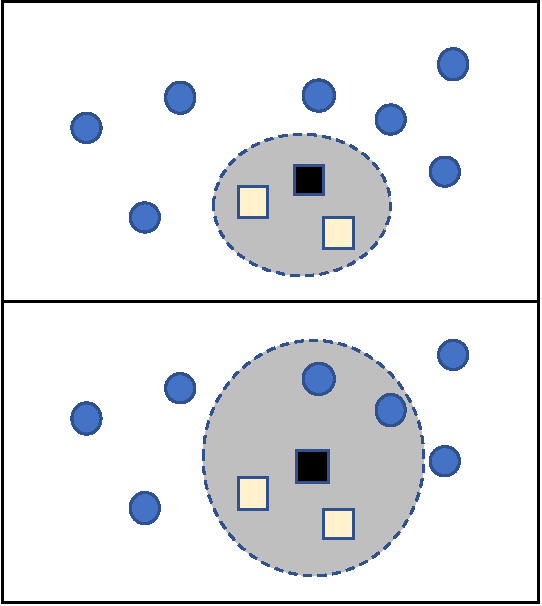
\includegraphics[width=1.5in]{imgs/bln/neighborhood.pdf}
    \caption{Unbalanced (top) and balanced (bottom) neighborhoods}
    \label{fig:neighbor}
\end{figure}

To enhance the degree of C-fairness in such a context, we introduce the notion of a \textit{balanced neighborhood}. A balanced neighborhood is one in which recommendations for all users are generated from neighborhoods that are balanced with respect to the protected and unprotected classes. This is shown in the bottom half of Figure~\ref{fig:neighbor}. The target has an equal number of peers inside and outside of the protected class. In the case of job recommendation discussed above, this would mean that female job seekers get recommendations from some female and some male peers.

There are a variety of ways that balanced neighborhoods might be formed. The simplest way would be to create neighborhoods for each user that balance accuracy against group membership. However, this would be highly computationally inefficient, requiring the solution of a separate optimization problem for each user. 

In this research, we explore an extension of the well-known Sparse Linear Method (SLIM)~\cite{ning2011slim}. SLIM is well-known as a state-of-the-art technology for collaborative recommendation. It is a generalization of item-based recommendation in which a regression coefficient is learned for each $\langle user, item \rangle$ pair. It can be slower to optimize than factorization-based methods, but for our purposes, it has the important benefit that the learned coefficients are readily interpretable with regard to group membership. Our extension of SLIM uses regularization to control the way different neighbors are weighted, with the goal of achieving balance between protected and non-protected neighbors for each user.

\subsubsection{\textbf{Sparse Linear Method}}
\hfill

SLIM learns $\langle user, item \rangle$ regression weights through optimization, minimizing a regularized loss function. Although this is not proposed in the original SLIM paper, it is possible to create a user-based version of SLIM (labeled SLIM-U in~\cite{zheng2014cslim}), which generalizes the user-based algorithm in the same way. 

Assume that there are $M$ users (a set $U$), $N$ items (a set $I$), and let us denote the associated 2-dimensional rating matrix by $R$. SLIM is designed for item ranking and therefore $R$ is typically binary. We will relax that requirement in this work, We use $u_i$ to denote user $i$ and $t_j$ to denote the item $j$. An entry, $r_{ij}$, in matrix $R$ represents the rating of $u_i$ on $t_j$.

SLIM-U predicts the ranking score $\hat{s}$ for a given user, item pair $\langle u_i, t_j \rangle$ as a weighted sum:

\begin{equation}
    \hat{s}_{ij} = \sum_{k \in U}{w_{ik}r_{kj}}, 
\end{equation}
where $w_{ii} = 0$ and $w_{ik} >= 0$.

Alternatively, this can be expressed as a matrix operation yielding the entire prediction matrix $\hat{S}$:    
\begin{equation}
\hat{S} = WR,
\end{equation}
where $W$ is an $M x M$ matrix of user-user weights. For efficiency, it is very important that this matrix be sparse.

The optimal weights for SLIM-U can be derived by solving the following minimization problem:

\begin{equation}
\mbox{min}_W \frac{1}{2}\left\Vert R - WR \right\Vert^2 + 
    \lambda_1 \left\Vert W \right\Vert^1 +
    \frac{\lambda_2}{2}\left\Vert W \right\Vert^2,   
\end{equation}
subject to $W > 0$  and $diag(W) = 0$.

The $\left\Vert W \right\Vert^2$ term represents the $\ell_2$ norm of the $W$ matrix and $\left\Vert W \right\Vert^1$ represents the $\ell_1$ norm. These regularization terms are present to constrain the optimization to prefer sparse sets of weights. Typically, coordinate descent is used for optimization. Refer to \cite{ning2011slim} for additional details. 

% \subsubsection{Neighborhood Balance}
\paragraph{\textbf{Neighborhood Balance}}

Recall that our aim in fair recommendation is to eliminate segregated recommendation neighborhoods where protected class users only receive recommendations from other users in the same class. Such neighborhoods would tend to magnify any biases present in the system. If users in the protected class only are recommended certain items, then they will be more likely to click on those items and thus increase the likelihood that the collaborative system will make these items the ones that others in the protected group see.

To reduce the probability that such neighborhoods will form, we use the SLIM-U formalization of the recommendation problem, but we add another regularization term to the loss function, which we call the \textit{neighborhood balance} term. To describe this term, we will enrich our notation further by indicating $U^+$ to be the subset of $U$ containing users in the protected class with the remaining users in the class $U^-$. Let $W_i^+$ be the set of weights for users in $U^+$ and $W_i^-$ be the corresponding set of weights for the non-protected class. Then the neighborhood balance term $b_i$ for a given user $i$ is the squared difference between the weights assigned to peers in the protected class versus the unprotected class.

\begin{equation}
    b_i = (\sum_{w^+ \in W_i^+}{w^+} - \sum_{w^- \in W_i^-}{w^-})^2
\end{equation}

A low value for the neighborhood balance term means that the user's predictions will be generated by weighting protected and unprotected users on a relatively equal basis.\footnote{Note that this is a class-blind optimization that tries to build balanced neighborhoods for both the protected and unprotected users. It is also possible to formulate the objective such that it only impacts the protected class and we leave this option for future work.}

Another way to express this idea is to create a vector $p$ of dimension $M$. If $u_i$ is in $U^+$, then $p_i = 1$; if $u_i$ is in $U^-$, then $p_i = -1$. Then, the sum expressed above can be rewritten as $b_i = (p^T \cdot w_i)^2$. By adding up this term for all users and adding it to the loss function, we can allow the optimization process to derive weights with neighborhood balance in mind. This adapted version of SLIM-U we will call \textit{Balanced Neighborhood SLIM-U} or BN-SLIM-U.

As in the case of the original SLIM implementation, we can apply the method of coordinate descent to optimize the objective. The full loss function is as follows:

\begin{equation}
\begin{split}
 L = \frac{1}{2}\left\Vert R - WR \right\Vert^2 + 
    \lambda_1 \left\Vert W \right\Vert^1 + 
    \frac{\lambda_2}{2}\left\Vert W \right\Vert^2 + \\
    \frac{\lambda_3}{2}\sum_{i \in U}\left(\sum_{k \in U}p_iw_{ik}\right)^2,
\end{split}
\end{equation}
where $w_{ii}=0$ and $w_{ik}>=0$ and where $\lambda_3$ is a parameter controlling the influence of the neighborhood balance calculation on the overall optimization

This loss function retains the property of the original SLIM algorithm in that the rows of the weight matrix are independent, and the weights in each row (those for each user) can be optimized independently. The algorithm chooses one $w_{ik}$ weight and solves the optimization problem for that weight, repeating over all the weights until convergence is reached. If we take the derivative of $L$ with respect to a single weight $w_{ik}$, we obtain

\begin{equation}\label{eq:derivative}
\begin{split}
\frac{\partial L_i}{\partial w_{ik}} = \sum_{j \in I}{(r_{ij} - 
    \sum_{l \in U'}{w_{il}r_{lj}})} + w_{ik}\sum_{j \in I}{r_{kj}^2} +  \\
    \lambda_1 + \lambda_2w_{ik} + \lambda_3p_k\sum_{l \in U'}{p_lw_{il}} 
\end{split}
\end{equation}
where $U' = U - \{u_i, u_k\}$.

We then set this derivative to zero and solve for the value of $w_{ik}$ that produces this minimum. This becomes the coordinate descent update step. 

\begin{equation}\label{eq:update}
\begin{split}
    w_{ik} \leftarrow \frac{S\left(X_{ik}, \lambda_1\right)_+}
    {\sum_{j \in I}{r_{kj}^2} + \lambda_2 + \lambda_3} \\
    X_{ik} = \sum_{j \in I}{(r_{ij} - 
    \sum_{l \in U'}{w_{il}r_{lj}})}+\lambda_3p_k\sum_{l \in U'}{p_lw_{il}}
\end{split}
\end{equation}
where $S()_+$ is the soft threshold operator defined in ~\cite{friedman_pathwise_2007}.

\paragraph{\textbf{Item-based neighborhoods}}

As noted above, some applications may require P-fairness: making the recommendation outcomes fair relative to the items being recommended. In our micro-finance example, the operators of this site have the goal of providing equal exposure to loans from different geographic regions. To address the P-fairness case, we can use an analogous approach using item neighborhoods and item weights, ensuring that items in a protected group are in neighborhoods that have balanced membership of items from the unprotected group. The derivation of the loss function is exactly analogous, yielding another variant of the SLIM algorithm that we refer to as \textit{Balanced Neighborhood SLIM} or BN-SLIM.

\subsubsection{\textbf{Methodology}}
\hfill

In order to evaluate our balanced neighborhood approach, we conducted separate sets of experiments in both consumer- and provider-fairness. It is very difficult to find datasets that contain the kind of features that would be necessary to evaluate fairness-aware recommendation algorithms, especially related to user demographics in sensitive application areas such as employment. 

For the purposes of this paper, we are using the well-known MovieLens 1M dataset~\cite{movielens}, which contains gender information for each user, as well as ratings of 4,000 movies by 6,000 users. Movie recommendation is, of course, a domain of pure individual taste and therefore not an obvious candidate for fairness-aware recommendation. Following the example of \cite{yao2017beyond}, our approach to construct an artificial equity scenario within this data for expository purposes only, with the understanding that real scenarios can be approached with a similar methodology. 

Our consumer-fairness scenario centers on movie genres. It can be seen in this data that there is a minority of female users (1709 out of the total of 6040). Certain genres display a discrepancy in recommendation delivery to male and female users. For example, in the ``Crime'' genre, female users rate a very similar number of movies (average of 0.048\% of female profiles vs 0.049\% of male profiles) and rate them similarly: an average rating of 3.7 for both female and male users. However, our baseline unmodified SLIM-U algorithm recommends in the top 10 an average of 1.10 ``Crime'' movies per female user as opposed to 1.18 such movies to male users. We are still exploring the cause of this discrepancy, but it seems likely that there are influential female users with a lower opinion of this genre. 

Given that the rating profiles are similar but the recommendation outcomes are different, we can therefore conclude that the female users experience a deprivation of ``Crime'' movies compared to their male counter-parts. Similar losses can be observed for other genres. We are not asserting that there is any harm associated with this outcome. It is sufficient that these differences allow us to validate the properties of the BN-SLIM-U algorithm.

Our goal, then, is to reduce or eliminate genre discrepancies with minimal accuracy loss by constructing balanced neighborhoods for the MovieLens users. The $p$ vector in Equation~\ref{eq:update} therefore will have a 1 for female users and a -1 for male users. In the experiments below, we compare the user-based SLIM algorithm in its unmodified form and the balanced neighborhood version BN-SLIM-U.

In evaluating fairness of outcome, we use a variant of what is known in statistics as \textit{risk ratio} or \textit{relative risk} (RR)\cite{romei2014multidisciplinary}. We measure what is effectively \textit{relative opportunity}. In other words, we measure the observed probability of protected class items being recommended divided by the probability of unprotected class items being recommended. In our MovieLens experiments, we measure the number of movies in protected and unprotected genres included in recommendation lists  as the measure of outcome quality. We construct a consumer-side equity score, $E_c@k$ for recommendation lists of k items, as the ratio between the outcomes for the different groups. Let $P_i@k = {\rho_1, \rho_2, ..., \rho_k}$ be the top $k$ recommendation list for user $i$, and let $\gamma()$ be a function $\rho \rightarrow \{0,1\}$ that maps to 1 if the recommended movie is in a protected genre. Then:

\begin{equation}
E_c@k=\frac{\sum_{i \in U^+}{\sum_{\rho \in P_i@k}{\gamma(\rho)}}/|U^+|}
{\sum_{i \in U^-}{\sum_{\rho \in P_i@k}{\gamma(\rho)}}/|U^-|}
\end{equation}

$E_c@k$ will be less than 1 when the protected group is, on average, recommended fewer movies of the desired genre. It may be unrealistic to imagine that this value should approach 1: the metric does not correct for other factors that might influence this score -- for example, female users may rate a particular genre significantly lower and an equality of outcome should not be expected. While the absolute value of the metric may be difficult to interpret, it is still useful for comparing algorithms. The one with the higher $E_c@k$ is providing more movies in the given genre to the protected group. Note that this is an additive, utilitarian measure of outcome equity and does not take into account variations in user experience. More nuanced measures of distributional equity, including Pareto improvement, we leave for future work.

As in any multi-criteria setting, we must be concerned about any loss of accuracy that results from taking additional criteria into consideration. Therefore, we also evaluate the ranking accuracy of our algorithms in the results below. The measure that we use is normalized discounted cumulative gain (NDCG) measured at a specific list length. In this measure, an item appearing on a recommendation list accrues ``gain'' according to its position on the list -- thus the discount. The measure is normalized by comparing the algorithm's performance to the best ranking that could have been achieved. 

Let $P_i@10$ be a list of retrieved list of length 10 and let $\tau$ be an indicator function that is 1 for movies that the user liked and 0 for others. Then, DCG@10 is computed as

\begin{equation}
DCG@10 = \sum_{k=1}^{10}{\frac{\tau(\rho_k)}{log_2(k+1)}}
\end{equation}

NDCG@10 is this DCG@10 value divided by the optimal DCG, which occurs when all of the movies liked by the user and appearing the test set are ranked at the top of the list in their order of preference.

\paragraph{\textbf{Provider fairness}}

To evaluate our approach for provider fairness, we are using a dataset extracted from the Kiva.org microlending site using the site's API\footnote{http://build.kiva.org/}. Again, we have constructed our own scenario using this data, focusing on geographic region. In our dataset, we find that there are some geographic regions with a higher than average number of unfunded loans. In these regions, borrowers have a lower probability of getting the desired capital. See Table~\ref{tab:unfunded}.

\begin{table}
    \centering
\begin{tabular}{l|l|r}
    Category & Region & Unfunded \% \\ \hline
    Unprotected & North America & 1.73 \\
    & Eastern Europe & 0.99 \\
    & South America & 4.33 \\
    & Asia & 6.70 \\ \hline
    Protected & Africa & 10.57 \\
    & Middle East & 13.23 \\
    & Central America & 8.81 \\
\end{tabular}
    \caption{Percentage of unfunded loans by region}
    \label{tab:unfunded}
\end{table}

For the purposes of our experiments, we will assume that one of the goals of a microlending site is to equalize access to capital across geographic regions. Kiva does not currently offer personalized recommendation of loans to its users, but if it did, a fairness-aware recommendation approach could be used to promote the loans of borrowers in the underserved regions. 

We will therefore treat the under-represented regions collectively as the protected group and the other regions as the unprotected group. This enables us to use our item-based neighborhood balance algorithm described above. A more fine-grained approach to geographic equity that tries to balance across all regions would require additional algorithmic development and is left for future work. 

Again, we will represent fairness as a ratio of outcomes. It is simpler to compute in this case, as we are not dividing the recommendations by genre. The provider-side equity score, $E_p@k$, is defined on recommendation lists of k items. Let $L^+$ be the set of loans in the test set that are from the protected regions, and $L^-$ be the corresponding set from the unprotected regions. Also, let $\pi^+()$ be an indicator function $\rho \rightarrow \{0,1\}$ that maps to 1 if the recommended loan is from a protected region and $\pi^-$ is a similar function for the unprotected regions. Then:

\begin{equation}
E_p@k=\frac{\sum_{i \in U}{\sum_{\rho \in P_i@k}{\pi^+(\rho)}}/|L^+|}
{\sum_{i \in U}{\sum_{\rho \in P_i@k}{\pi^-(\rho)}}/|L^-|}
\end{equation}

$E_p@k$ will be less than 1 when loans from the protected regions are appearing less often on recommendation lists. As with $E_c$, this is a utilitarian measure, summing over all borrower regions, and does not speak to the the distribution across individual borrowers. Like $E_c$, it does not take the rank of recommended items into account.

\subsubsection{\textbf{Results}}
\hfill

We implemented the SLIM-U, BN-SLIM, and BN-SLIM-U algorithms using LibRec 2.0~\cite{guo2015librec}, and used its existing implementation of SLIM. We used 5-fold cross-validation as implemented within the library.

\paragraph{\textbf{Consumer fairness: MovieLens}}

Within the MovieLens 1M dataset, we selected the five genres on which the SLIM-U algorithm produced the lowest equity scores: ``Film-Noir'', ``Mystery'', ``Horror'', ``Documentary'', and ``Crime''. The parameters were set as follows: $\lambda_1 = 0.1$, $\lambda_2 = 0.001$, and (for BN-SLIM-U) $\lambda_3 = 25$\footnote{Because the balance term measures the difference in weights, it tends to be much smaller than the terms that measure the sums of weights. Therefore, the regularization constant must be much higher for the balance term to have an impact on the optimization.}. 

\begin{figure}[tbh]
    \centering
    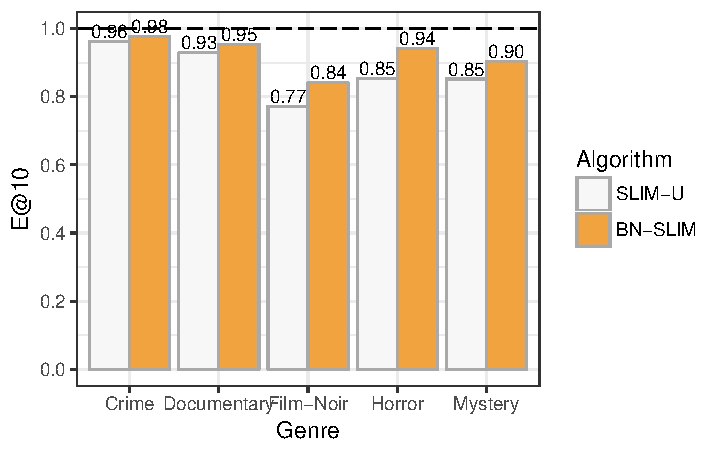
\includegraphics[width=3.00in]{imgs/bln/genre-compare3.pdf}
    \caption{Equity score for SLIM-U and BN-SLIM-U. Line indicates equal percentage across genders}
    \label{fig:genre}
\end{figure}

Figure~\ref{fig:genre} shows the results of the experiment in terms of the equity scores for each genre. Perfect equity (1.0) is marked with the dashed line. As we can see, in every case, the balanced neighborhood algorithm produced an equity score closer to 1.0 than the unmodified algorithm. The largest jump is seen in the ``Horror'' genre, about 0.09 in the equity score or around 10\%.

In terms of accuracy, there was only a small loss of NDCG@10 between the two conditions. See Table~\ref{tab:ndcg}. The difference amounts to approximately 2\% loss in NDCG@10 for the balanced neighborhood version.

\begin{table}
\centering
\begin{tabular}{c|c}
    Algorithm &  NDCG@10 \\ \hline
    SLIM-U & 0.053 \\ \hline
    BN-SLIM & 0.052 \\ \hline
\end{tabular}
\caption{Ranking accuracy}
\label{tab:ndcg}
\end{table}

Because the balanced neighborhood algorithm is applied across all users, it also has the effect of showing male users movie genres that occur more frequently for female users. To see this effect, we examined the five genres with the highest $E_c@10$ values: ``Fantasy'', ``Animation'', ``War'', ``Romance'', and ``Western'' using the same parameter values as above. The results appear in Figure~\ref{fig:inverse-equity} and show a similar result. ``War'' is something of an anomaly here, both because it is perhaps unexpected to see it as a one of the more female-recommended genres and because the genre-balance algorithm pushes it to become more skewed rather than less. We are investigating the cause of this phenomenon. Overall, the BN-SLIM-U algorithm produces a recommendation experience in which the occurrence of gender-specific genres is more closely equalized, with small loss in ranking accuracy. 

\begin{figure}[bth]
    \centering
    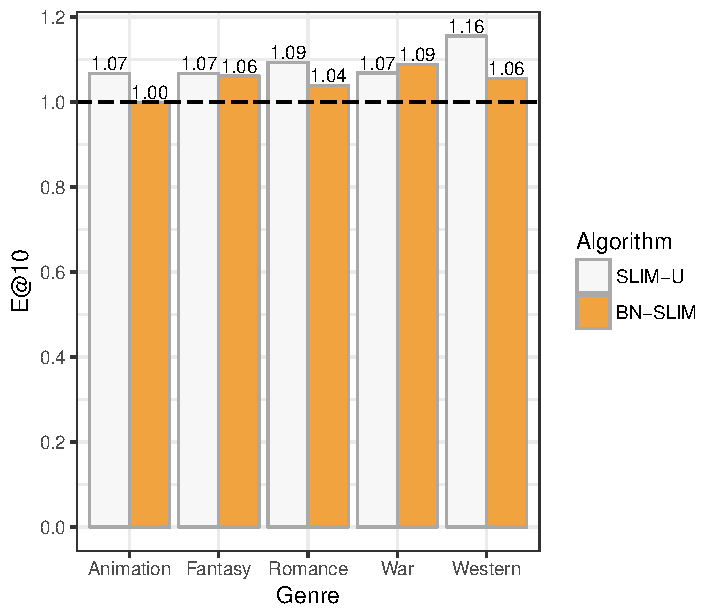
\includegraphics[width=3in]{imgs/bln/inverse-genres3.pdf}
    \caption{Equity scores for female-preferred genres}
    \label{fig:inverse-equity}
\end{figure}

\paragraph{\textbf{Provider fairness: Kiva.org}}
Our dataset was extracted from Kiva's public API in September of 2016 and contains approximately 1 million loans funded by approximately 180,000 lenders. One challenge for collaborative recommendation in the microlending area is that loans are generally one-time endeavors. Unlike a movie that can be watched by an unrestricted number of viewers, a loan -- once funded -- disappears from Kiva.org and is not available for other lenders to view or support. Most loans are supported by from 1-330 lenders, by contrast, a popular movie in the MovieLens dataset might be rated by thousands of users. Thus, the lender-borrower relation is highly sparse, and loans have very small profiles.

To be able to apply the SLIM algorithm, we used a hybrid recommendation technique incorporating content data in the form of loan characteristics. We characterized each loan using five characteristics available from Kiva: borrower gender, borrower country, loan sector, loan purpose, and loan amount. Each of the original 1 million loan identifiers in the database was replaced with a psuedo-item identifier corresponding to the appropriate combination of loan characteristics. A 5-core transformation was then applied to the dataset, retaining only those users who had funded at least 5 psuedo-items and those psuedo-items with at least 5 funders. The retained dataset has 3,593 psuedo-items, 29,342 users and 393,035 ratings.

Kiva.org divides its borrowers into 9 geographic regions. As discussed above, for the purposes of this paper we are defining the protected group as those regions of the world where it appears to be more difficult to fund loans. (In Kiva.org, a loan that does not attract enough lenders over a 30 day period is marked as unfunded and dropped from the system.) As shown in Table~\ref{tab:unfunded}, the regions of North America, Eastern Europe, South America, and Asia have proportionately more funded loans than the regions of Africa, Middle East, and Central America\footnote{Our data set had only a single loan request from Australia.}. These regions where borrowers have lower funding percentages are treated as the protected group in our experiments.

With this transformation in place, it was possible to apply the SLIM algorithm and generate personalized recommendations. The regularization parameters were set as follows: $\lambda_1 = 0.01$ and $\lambda_2 = 0.001$. For BN-SLIM, $\lambda_3$ had a value of 0.9. Table~\ref{tab:results} shows the performance of the these algorithms in the provider fairness condition. Interestingly, the ranking accuracy, as measured by NDCG@10, actually increases between the conditions, indicating that the balanced neighborhood condition actually yields better recommendation lists than the unmodified SLIM algorithm. In addition, the $E_p@10$ value, which is unbalanced at 0.90 for SLIM is improved to close to 1.0, the equity target that we were aiming for.

\begin{table}
    \centering
\begin{tabular}{l|r|r}
    Algorithm & NDCG@10 & $E_p@10$ \\ \hline
    SLIM & 0.046 & 0.90 \\ \hline
    BN-SLIM & 0.049 & 1.05 \\ \hline
\end{tabular}
    \caption{Comparison of algorithm performance}
    \label{tab:results}
\end{table}


% \subsubsection{\textbf{Close Related Work}}
% There has been relatively little work on fairness in recommender systems.
% Most researchers in the area have defined fairness in terms of differing levels of accuracy for different classes of users. See, for example, \cite{DBLP:conf/recsys/KamishimaAAS14,kamisha-akaho-fatrec-2017,yao_huang_fatml-2017}. 

% As noted above, some special cases of provider-side fairness have been studied in the context of diversity-aware and long-tail recommendation. See, for example, \cite{Zhang:2008:AMI:1454008.1454030,adomavicius2012improving,o2004preserving,adomavicius2012improving}. 
% Our BN-SLIM algorithm can be seen as an approach to building systems that target particular diversity-aware recommendation problems, where the providers and/or items can be divided into two disjoint categories. However, the approach is particularly suited to fairness-aware contexts because the objective function is optimized precisely when the protected and unprotected groups are weighted the same by the algorithm. 

% The most obvious precursor for this research is the work of Dwork et al. in the area of fair representation~\cite{zemel2013learning,fairness}. The authors propose learning a mapping between the individual instances in the data to prototype instances with balanced membership such that protected group identities are not recoverable. Our application of this concept is different in that we are building on the standard nearest neighbor techniques in recommender systems and building balanced neighborhoods to ensure diversity among the peers from whom recommendations are generated. 

\subsubsection{\textbf{Conclusion and Future Work}}

% This paper extends ideas of fairness in classification to personalized recommendation. 
Our BN-SLIM algorithm can be seen as an approach to building systems that target particular diversity-aware recommendation problems, where the providers and/or items can be divided into two disjoint categories. However, the approach is particularly suited to fairness-aware contexts because the objective function is optimized precisely when the protected and unprotected groups are weighted the same by the algorithm. 

The most obvious precursor for this research is the work of Dwork et al. in the area of fair representation~\cite{zemel2013learning,fairness}. The authors propose learning a mapping between the individual instances in the data to prototype instances with balanced membership such that protected group identities are not recoverable. 

This paper extends this idea of fairness in classification to personalized recommendation. However, our application of this concept is different in that we are building on the standard nearest neighbor techniques in recommender systems and building balanced neighborhoods to ensure diversity among the peers from whom recommendations are generated. 

A key aspect of this extension is to note the tension between a personalized view of recommendation delivery and a regulatory view that values particular outcomes. The regulatory view is somewhat foreign to research in personalization, but there are strong arguments that total obedience to user preference is not always risk-free or desirable~\cite{pariser2011filter,sunstein2009republic}. This paper also introduces the concept of multisided fairness, relevant in multisided platforms that serve a matchmaking function. We identify consumer- and provider- fairness as properties desirable in certain applications and demonstrate that the concept of balanced neighborhoods in conjunction with the well-known sparse linear method can be used to balance personalization with fairness considerations.

In our future work, we plan to extend these findings in several ways. It is possible that a multisided platform may require fairness be considered for both consumers and providers at the same time: a CP-fairness condition. For example, a rental property recommender may treat minority applicants as a protected class and wish to ensure that they are recommended properties similar to unprotected renters. At the same time, the recommender may wish to treat minority landlords as a protected class and ensure that highly-qualified tenants are referred to them at the same rate as to landlords who are not in the protected class. One important question for future research is how the outcomes for each stakeholder and the overall system performance are affected by combining consumer- and provider-fairness concerns.
Another path to pursue is to have a more extensive experimentation of the fairness properties of the balanced neighborhood SLIM for both consumers and providers. We would like to test this idea on K-nearest neighbor method as well. Finally, we expect to publish a journal article of these thorough experiments in the Information and Management Journal.

% Another important area of research is to extend our measures of fairness. The additive measures used in this paper capture an aggregate representation of how recommendation results are changing for user and provider groups generally, but they do not permit fine-grained analysis of the tradeoffs experienced by individual users or providers. We do not know, for example, if the results of our Kiva.org experiments represent a Pareto improvement in system performance or just an average improvement over the stakeholder groups, and whether some subgroups are impacted more than others.

% One of the key challenges in this area is the domain-specificity of recommendation environments. The utilities that are delivered to each class of stakeholder are highly dependent on the type of item being recommended, the social function of the platform, and the interactions that it enables. It is therefore difficult to find appropriate data sets for experimentation and challenging to generalize across recommendation scenarios. 

